\section{¿Cómo vamos a trabajar?}

Vamos trabajar dentro de un proyecto Java de tipo Maven, por lo tanto, es necesario instalar soporte Java, particularmente el \emph{plug--in \textbf{Maven for Java}} (\verb|vscjava.vscode-maven|).  Para más información, ver la documentación \href{https://code.visualstudio.com/docs/java/java-project}{\emph{Java Project Management in VS Code}} de la página de Visual Studio Code.

\begin{figure}[p]
	\centering
	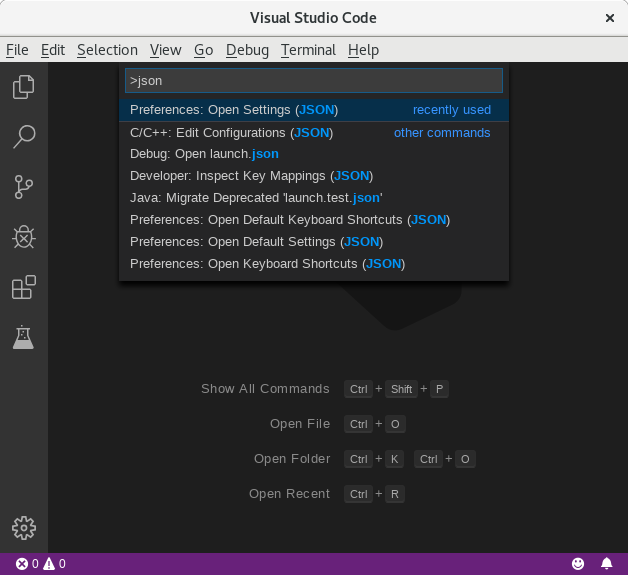
\includegraphics[width=.95\textwidth]{img/SelectJSON}
	\caption{Acceso a la configuración (archivo \texttt{settings.json}).}
	\label{preferences}
\end{figure}

Para simplificar la generación del software, vamos a colocar todos los archivos \verb|.java| en el mismo paquete que la aplicación.  Igualmente, algunos archivos de salida de ANTLR se guardarán en la carpeta \verb|.antlr|.  Para modificar el archivo \verb|settings.json|, se puede acceder de varias formas, pero la más simple es siguiendo estos pasos:
\begin{enumerate}
	\item Abrir el \emph{Command Palette} con \verb|Ctl+Shift+P|,
	\item Buscar la opción \emph{Preferences: Open Settings (JSON)} y seleccionarla (Figura~\ref{preferences}),
	\item Agregar las siguientes líneas de código
	\begin{lstlisting}[style=miJSON]
	"antlr4.generation.mode": "external",
	"antlr4.generation.visitors": true
	\end{lstlisting}
\end{enumerate}
Hay que tener en cuenta que la coma es el separador en JSON y no debe faltar.  Además, las líneas de código deben estar antes de la llave de cierre como en el ejemplo del Código~\ref{settings}.

\lstinputlisting[float,style=miJSON,caption={Ejemplo de archivo \texttt{code/settings.json}.},label=settings]{code/settings.json}

Si no incluimos el \verb|.jar| de ANTLR en el proyecto, debemos configurar el proyecto para que se pueda utilizar la biblioteca del sistema.  En el archivo \verb|.classpath| debemos agregar la línea
\begin{lstlisting}[style=miXML]
<classpathentry kind="lib"
    path="/usr/share/java/antlr-4.x.x-complete.jar" />	
\end{lstlisting}
donde \verb|"/usr/share/java/antlr-4.x.x-complete..jar"| es para Debian~9 y deben reemplazarla por lo que corresponda.  El archivo de ejemplo completo puede verse en el Código~\ref{classpath}.

\lstinputlisting[float,style=miXML,caption={Ejemplo de archivo \texttt{.classpath}.},label=classpath]{code/classpath}


\section{Primer Proyecto}
\label{primerproyecto}

Ya instalados y configurados los \emph{plug--ins} necesarios, podemos comenzar el primer proyecto.

\subsection{Crear Proyecto Java}
\label{proyecto_java}

\begin{figure}[t]
	\centering
	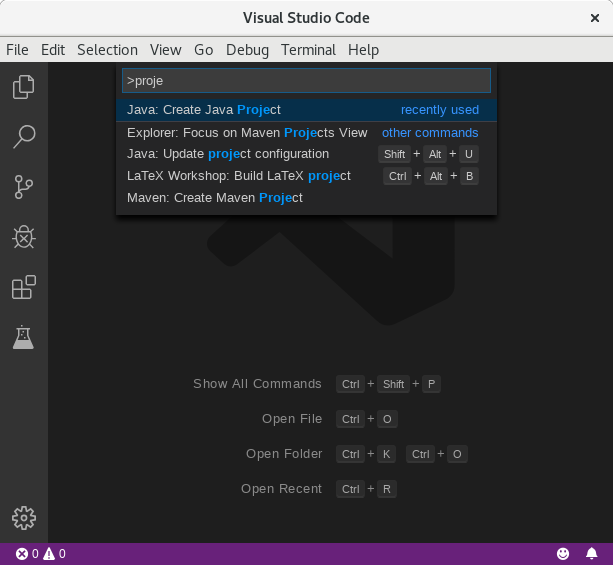
\includegraphics[width=.95\textwidth]{img/NuevoProyecto}
	\caption{Nuevo proyecto Java.}
	\label{maven_nuevo}
\end{figure}


El primer paso es crear un proyecto Java.  Para esto, se puede acceder al \emph{Command Palette} con el atajo \verb|Ctl+Shift+P|, escribir la palabra \emph{project} y elegir la opción ``\emph{Java: Create Java Project}'' (Fig.~\ref{maven_nuevo}). Luego, elegir la carpeta destino y darle nombre al proyecto.  Al finalizar estos pasos, tendremos un proyecto Java con un paquete por defecto denominado \verb|App|.  El archivo \verb|app.java| contiente el método \verb|main()| y está listo para compilar y ejecutar.


\begin{figure}[t]
	\centering
	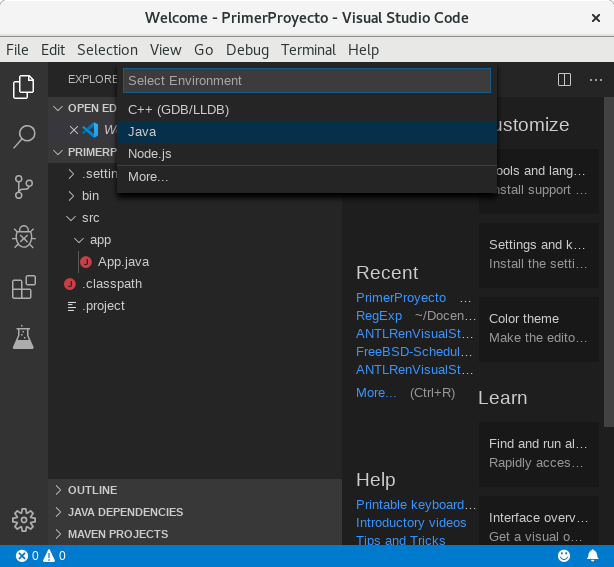
\includegraphics[width=.95\textwidth]{img/PrimerCompilacion}
	\caption{Elegir Java para compilar.}
	\label{java_project}
\end{figure}

\begin{figure}[t]
	\centering
	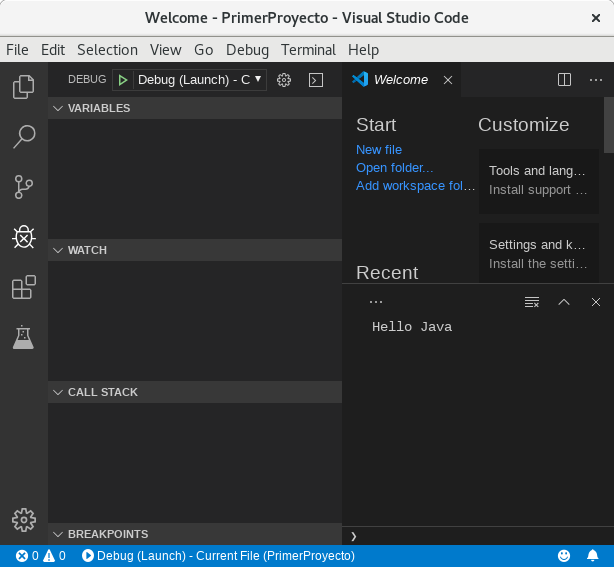
\includegraphics[width=.95\textwidth]{img/PrimeraEjecucion}
	\caption{Ejecutar el proyecto Java.}
	\label{hello_java}
\end{figure}


Recordemos que Visual Studio Code está pensado para desarrollar software, por lo tanto, cuando querramos ejecutar nuestro software vamos a hacerlo sobre el \emph{debugger}.  La ejecución se realiza presionando \verb|F5|.  La primera ejecución del proyecto necesita que se configuren parámetros de compilación qué, para nuestro caso, será suficiente con las configuraciones por defecto.  Al presionar \verb|F5| por primera vez debemos elegir ``Java'' como tipo de proyecto  (Fig.~\ref{java_project}).  Esta acción crea y abre el archivo de configuración \verb|launch.json| en la carpeta \verb|.vscode| del proyecto.  Si presionamos nuevamente \verb|F5| se ejecutará el proyecto y veremos que se abre el panel del \emph{debugger} y se muestra la salida por la \emph{debug console} con el texto ``\emph{Hello Java}'' (Fig.~\ref{hello_java}).  Las próximas veces se ejecutará nuestro programa sin necesidad de realizar configuraciones adicionales.

Finalmente, es necesario modificar el archivo \verb|launch.json| para habilitar la visualización del árbol sintáctico (para más información ver la guía del \emph{plug--in} ANTLR \href{https://github.com/mike-lischke/vscode-antlr4/blob/master/doc/grammar-debugging.md}{\emph{Debugging ANTLR4 grammars}}).  Se debe agregar a la lista de opciones la entrada del Código~\ref{launch_json_antlr}.

\lstinputlisting[float,style=miJSON,caption={Entrada en archivo \texttt{settings.json} para ANTLR.},label=launch_json_antlr]{code/launchJsonAntlr.json}

Para el correcto funcionamiento de ANTLR en nuestro proyecto es necesario ajustar del Código~\ref{launch_json_antlr} las entradas:
\begin{description}
	\item[\texttt{input}] el archivo de entrada a \emph{parsear},
	\item[\texttt{startRule}] el símbolo inicial,
	\item[\texttt{grammar}] (opcional) el archivo ANTLR con las reglas gramaticales,
	\item[\texttt{actionFile}] (opcional) ver documentación.
\end{description}

\subsection{Crear Proyecto Java con Maven}
\label{proyecto_maven}



\href{https://maven.apache.org/}{sitio web de Maven}

\href{https://maven.apache.org/guides/getting-started/maven-in-five-minutes.html}{guía rápida sobre Maven}


